\documentclass[tikz,border=10pt]{standalone}
%\usepackage[T1]{fontenc}
\usepackage[utf8]{inputenc}

\usepackage{amsmath}
\usepackage{amsfonts}
\usepackage{amssymb}
\usepackage{mathtools}

\usepackage{graphics}

\usepackage{tikz}
\usetikzlibrary{calc}
\usetikzlibrary{arrows}
\usetikzlibrary{positioning}

\definecolor{light-gray}{gray}{0.95}

\begin{document}
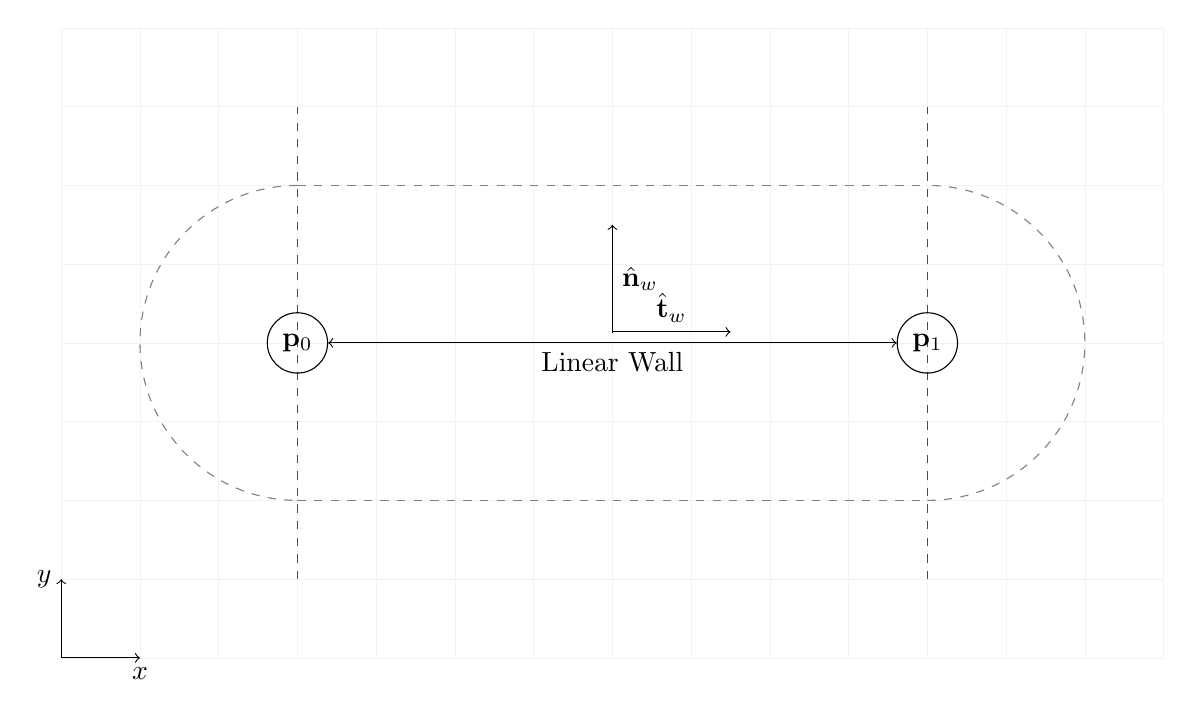
\begin{tikzpicture}
% Grid (x, y)
\coordinate[] (p1) at (-7, -4);
\coordinate[] (p2) at ( 7,  4);
\draw[help lines, step=1, light-gray] (p1) grid (p2);

\coordinate[] (xp) at ($ (p1) + (1, 0) $);
\coordinate[] (yp) at ($ (p1) + (0, 1) $);
\node[anchor=north] (x) at (xp)  {$ x $};
\node[anchor=east] (y) at (yp) {$ y $};
\draw[<->] (xp) -- (p1) -- (yp);

% ---------------------------------------------------
% Start - End - Mid - nodes
\coordinate[] (p0) at (-4, 0);
\coordinate[] (p1) at ( 4, 0);

% Vertical Lines
\draw[dashed, gray] ($ (p0) + (0,  2) $) -- ($ (p1) + (0,  2) $);
\draw[dashed, gray] ($ (p0) + (0, -2) $) -- ($ (p1) + (0, -2) $);
% Arcs
\draw[dashed, gray] ($ (p0) + (0,  2) $) arc (90:270:2);
\draw[dashed, gray] ($ (p1) + (0, -2) $) arc (-90:90:2);
% Horizontal Line - Separator
\draw[dashed, red] ($ (p0) + (0, -3) $) -- ($ (p0) + (0,  3) $);
\draw[dashed, red] ($ (p1) + (0, -3) $) -- ($ (p1) + (0,  3) $);
% Linear wall
\node[circle, draw] (start) at (p0) {$ \mathbf{p}_{0} $};
\node[circle, draw] (end) at (p1) {$ \mathbf{p}_{1} $};
\node[] (mid) at ($ (p0) + (p1) $) {};  % / 2
\path[] (start) edge[<->] node[below, midway]{Linear Wall} (end);
% Normal
\path[] (mid)
        edge[->] node[right, midway]{$ \hat{\mathbf{n}}_{w} $} 
        ($ (mid) + (0, 1.5) $);
% Tangent
\path[] ($ (mid) + (0, 0.14) $) 
        edge[->] node[above, midway]{$ \hat{\mathbf{t}}_{w} $} 
        ($ (mid) + (1.5, 0.14) $);
% ---------------------------------------------------
\end{tikzpicture}
\end{document}